\graphicspath{{figures/modeling/gearTrain/}}
\section{Modeling of the Gear System}\label{sec:ModGearSys}
In this section, the gear system will be modeled. 

\todo [inline,author=Geoff]{Work on intro and maybe put figure}


Three transfer functions are going to be determined in this section. First, the transfer of the motor's angular velocity $\omega_m$ to the angle of the arm $\theta_a$ through the gears. Then, two transfer functions are needed for $\tau_l$: the torque of the load comes from both the torque of the arm and stick $\tau_{as}$ and the frictions generated by the gears.


\subsection{Relation between $\Omega_m$ and $\Theta_a$}

\begin{figure}[htbp]
	\centering
	
\includegraphics[width=1\textwidth]{figures/FigureIsComing.PNG}
	\caption{Body diagram of the motor wheel system}
	\label{fig:Belt&Pulley}
\end{figure}

\startexplain
\explain{$J_m$ is the moment of inertia of the motor}{\si{\kilogram\meter\squared}}
\explain{$J_w$ is the moment of inertia of the wheel}{\si{\kilogram\meter\squared}}
\explain{$\omega_m$ is the motor's angular velocity}{\si{\meter\per\second}}
\explain{$\tau_m$ is the torque of the motor}{\si{\newton\meter}}
\explain{$F_1$ is the force transferred from the motor to the wheel}{\si{\newton}}
\explain{$r$ is the radius of the motor's wheel}{\si{\meter}}
\explain{$R$ is the radius of the wheel}{\si{\meter}}
\explain{$\tau_f$ is the torque of the gear train friction}{\si{\newton\meter}}
\explain{$\tau_L$ is the torque of the wheel's load}{\si{\newton\meter}}
\explain{$b_w$ is the viscous friction coefficient of the wheel}{\si{\newton\meter\per\radian\per\second}}
\stopexplain


From \autoref{fig:Belt&Pulley}, considering the small wheel as the one connected to the motor, if the motor shaft turns, the belt joining the small and the big wheel will make them turn the same distance:
\begin{equation}
	\theta_m r = \theta_w R \addunit{\meter}
\end{equation}

This expression is then differentiated to find the relation with the angular velocities:
\begin{equation}
	\omega_m r = \omega_w R\addunit{\meter\per\second}
	\label{eq:AngularVelRelation}
\end{equation}

Then the gear ratio can be defined as: 
\begin{equation}
	N = \frac{r}{R} \addunit{1}
	\label{eq:GearRatio}
\end{equation}

As the gear system is composed by three similar connected wheels structures like shown in \autoref{fig:Belt&Pulley}, the ratio between small wheel x, $r_x$, and big wheel x, $R_x$ is the same:
\begin{equation}
	\frac{r_x}{R_x} = \frac{r_{motor}}{R_{w_1}} = \frac{r_{w_1}}{R_{w_2}} = \frac{r_{w_2}}{R_{w_3}} = N \addunit{1}
\end{equation}

Knowing this and since $\omega_m$ is transferred through three gears, the relation between the angular velocity of the motor $\omega_m$ and the angle of the arm $\theta_a$ is found following the principle of \autoref{eq:AngularVelRelation}:
\begin{subequations} \label{eq:tech_ToA}
	\begin{flalign}
		&\omega_a(t) = N^3 \omega_m(t) \\
		&\theta_a(t) = N^3 \int_{0}^{t}\omega_m(v) dv \\
		&\mathcal{L}\{\theta_a(t)\} = \Theta_a(s) = N^3 \cdot \frac{1}{s} \Omega_m(s) \addunit{1}
	\end{flalign}
\end{subequations}

The transfer function from the motor's angle velocity to the angle of the arm is:
\begin{equation}\label{eq:thetaOmega}
	\frac{\Theta_a(s)}{\Omega_m(s)} =  \frac{N^3}{s} \addunit{1}
\end{equation}

\subsection{Linear Model}
\todo[inline,author=Geoff]{Why linear model?}

In order to design an effective feedback control system a linear model is a necessity. As seen previously in \autoref{eq:thetaOmega} $\frac{\Theta_a(s)}{\omega_m(s)}$ is already a linear relationship. So in order to get a linear system only the transfer function $\frac{\omega_m(s)}{U(s)}$ has to be linearized.

It can be seen from \autoref{eq:DCMotorTFWithLoad}, that in order to linearize $\frac{\omega_m(s)}{U(s)}$ $\tau_l$ has to be rewrite in function of $U(s)$ and $\omega_m(s)$.

\subsection{Determining $\tau_l$}
As said in \autoref{sec:ModGearSys} $\tau_l(s)$ is the torque of the load. In the inverted pendulum case the load is composed of the friction and the torque necessary to counter the gravity which result in \autoref{eq:TauL}.

\begin{equation}\label{eq:TauL}
	\tau_l = \tau_{f_{gear}} + \tau_{as} \addunit{\newton\meter}
\end{equation}

It is necessary then to derive $\tau_{f_{gear}}$ and $\tau_{as}$ to see if they are requiring linearization.


\subsubsection*{Determining $\tau_{f_{gear}}$}
The gear train is composed by three identical belt and pulley system. \autoref{fig:Belt&Pulley} corresponds to the first system between the motor and the first wheel. 

Using the previously stated $2^{nd}$ law of motion, the mechanical equation for the motor wheel can be found from \autoref{fig:MotorBodyDiagram}:

\begin{equation}
    J_m \dot{\omega}_m = \tau_m + F_1r - b_m\omega_m \addunit{\newton\meter}
    \label{eq:MotorfreeBody}
\end{equation}

For the body diagram for the wheel in \autoref{fig:Belt&Pulley}:
\begin{equation}
	J_w\dot{\omega}_w = -F_1R -\tau_L -b_w\omega_w \addunit{\newton\meter}
\end{equation}

Looking at the whole gear train, $\tau_{f_{gear}}$ represents the total friction and $\tau_L$ is the opposite of the torque transferred to the next wheel. Which gives for wheels 1, 2 and 3:

\begin{subequations} 
	\begin{flalign} \label{eq:GiveMeAnOriginalName}
		&J_{w_1}\dot{\omega}_{w_1} = -F_1R + F_2r -b_{w_1}\omega_{w_1} \addunit{\newton\meter}\\ 
		&J_{w_2}\dot{\omega}_{w_2} = -F_2R + F_3r -b_{w_2}\omega_{w_2} \addunit{\newton\meter}\\ 
		&J_{w_3}\dot{\omega}_{w_3} = -F_3R - b_{w_3}\omega_{w_3} \addunit{\newton\meter}
	\end{flalign}
\end{subequations}

Using the relation in \autoref{eq:AngularVelRelation}, the angular velocity of each wheels can be found according to $\omega_m$:
\begin{subequations} 
	\begin{flalign}
		&\omega_{w_1} = N \omega_m \addunit{\radian\per\second}\\
		&\omega_{w_2} = N \omega_{w_1} = N^2 \omega_m \addunit{\radian\per\second}\\
		&\omega_{w_3} = N \omega_{w_2} = N^3 \omega_m \addunit{\radian\per\second}
	\end{flalign}
\end{subequations}

The same equations are valid with angular accelerations.
Which gives for Equations \ref{eq:GiveMeAnOriginalName}:
\begin{subequations} 
	\begin{flalign}  
		&J_{w_1}N\dot{\omega}_m = -F_1R + F_2r -b_{w_1}N\omega_m \addunit{\newton\meter}\\ 
		&J_{w_2}N^2\dot{\omega}_m = -F_2R + F_3r -b_{w_2}N^2\omega_m  \addunit{\newton\meter}\\ 
		&J_{w_3}N^3\dot{\omega}_m = -F_3R - b_{w_3}N^3\omega_m  \addunit{\newton\meter}
	\end{flalign}
\end{subequations}

The total friction torque $\tau_{f_{gear}}$ in the gear train is the torque that needs to be overcome by the torque of the motor in order to make the gear train move. It means that when the gear train is static:

\begin{subequations} \label{eq:findTauf}
	\begin{flalign}
		&\omega_m = \SI{0}{\radian\per\second}\\
		&\tau_m \leqslant \tau_{f_{gear}} \addunit{\newton\meter}
	\end{flalign}
\end{subequations}

To find $\tau_{f_{gear}}$, the special case where $\tau_m = \tau_{f_{gear}}$ is studied. Inserting \autoref{eq:findTauf} into \autoref{eq:MotorfreeBody}:

\begin{equation} 
		\tau_{f_{gear}} = -F_1 \cdot r \addunit{\newton\meter}
		\label{eq:TaufF1r}
\end{equation}

$F_1$ needs to be isolated from \autoref{eq:GiveMeAnOriginalName}. Each forces $F_1$, $F_2$ and $F_3$ are then isolated, giving: 

\begin{subequations} 
	\begin{flalign}
		&F_1 = -\frac{1}{R} (b_{w_1}N\omega_m + J_{w_1}N\dot{\omega}_m - F_2r) \addunit{\newton} 	\label{eq:F1}\\ 
		&F_2 = -\frac{1}{R} (b_{w_2}N^2\omega_m +  J_{w_2}N^2\dot{\omega}_m - F_3r) \addunit{\newton}	\label{eq:F2}\\
		&F_3 = -\frac{1}{R} (b_{w_3}N^3\omega_m + J_{w_3}N^3\dot{\omega}_m)	\addunit{\newton}		\label{eq:F3}
	\end{flalign}
\end{subequations}

Inserting \autoref{eq:F3} in \autoref{eq:F2}, then \autoref{eq:F2} in \autoref{eq:F1}, the expression of $F_1$ according to the friction and moment of inertia of each wheel is found:

\begin{flalign}
	F_1 = &-\frac{1}{R} N(b_{w_1}\omega_m + J_{w_1}\dot{\omega}_m \notag \\
	& +\frac{r}{R} N^2(b_{w_2}\omega_m + J_{w_2}\dot{\omega}_m \notag \\
	& +\frac{r}{R} N^3(b_{w_3}\omega_m + J_{w_3}\dot{\omega}_m))) \addunit{\newton}
\end{flalign}


Using \autoref{eq:TaufF1r} and the gear ratio in \autoref{eq:GearRatio}, the total friction is given by: 
\begin{align} \label{eq:TaufTimeDomain}
	\tau_{f_{gear}} =&\ N^2 (b_{w_1}\omega_m + J_{w_1}\dot{\omega}_m \notag \\
	& +N^3 (b_{w_2}\omega_m + J_{w_2}\dot{\omega}_m \notag \\
	& +N^4 (b_{w_3}\omega_m + J_{w_3}\dot{\omega}_m))) \addunit{\newton\meter}
\end{align}


\autoref{eq:TaufTimeDomain} is Laplace-transformed:

\begin{flalign} \label{eq:TaufLaplaceDomain}
	\mathcal{L}\{\tau_{f_{gear}}(t)\} = \tau_{f_{gear}}(s) = &\ N^2 (B_{w_1}\Omega_m + sJ_{w_1}\Omega_m \notag \\
	& +N^3 (B_{w_2}\Omega_m + sJ_{w_2}\Omega_m \notag \\
	& +N^4 (B_{w_3}\Omega_m + sJ_{w_3}\Omega_m))) \addunit{1}
\end{flalign}


\autoref{eq:TaufLaplaceDomain} is reorganized to find the final expression for $\tau_{f_{gear}}$ in \autoref{eq:TaufReorganized}:
\begin{equation}
	\tau_{f_{gear}} = \left[(N^2 J_1 + N^3 J_2 + N^4 J_3)s +( N^2 B_1 + N^3 B_2 + N^4 B_3)\right]\Omega_m \addunit{1}
	\label{eq:TaufReorganized}
\end{equation}











\subsubsection*{Determining $\tau_{as}$}

$\tau_{as}$ is the torque necessary for the motor to counter the load applied by the arm and the stick. It can be divided into two parts as in \autoref{eq:TauasBegin}.

\begin{equation}\label{eq:TauasBegin}
	\tau_{as}=\tau_a+\tau_s \addunit{\newton\meter}
\end{equation}
\startexplain
\explain{$\tau_a$ is the load of the arm}{\si{\newton\meter}}
\explain{$\tau_s$ is the load of the stick}{\si{\newton\meter}}
\stopexplain

The first part is the torque to counter the load of the arm, $\tau_a$. It is subjected to two torques as explained in \autoref{eq:TauAdef}.

\begin{equation}\label{eq:TauAdef}
	\tau_a=\tau_{a_{gravity}}+\tau_{a_{momentum}} \addunit{\newton\meter}
\end{equation}

 $\tau_{a_{gravity}}$ is the torque generated by the gravity. It is decided to approximate this torque by defining the arm as a pendulum with a weightless rod and all its mass is on the GC as a point. This approximation gives \autoref{eq:tauAgrav}.

\begin{equation}\label{eq:tauAgrav}
	\tau_{a_{gravity}}=-M_a\cdot g \cdot \frac{l_a}{2} sin(\Theta_a) \addunit{\newton\meter}
\end{equation}
\startexplain
\explain{$M_a$ is the mass of the arm}{\si{\kilogram}}
\stopexplain

$\tau_{a_{momentum}}$ is the torque of the momentum of the arm when it moves. This can be translated by the \autoref{eq:ArmMomentum}.

\begin{equation}\label{eq:ArmMomentum}
	\tau_{a_{momentum}}=\dot\omega_a\ \cdot J_a \addunit{\newton\meter}
\end{equation}
\startexplain
\explain{$J_a$ is the moment of inertia of the arm}{\si{\kilogram\meter\squared}}
\stopexplain

$\tau_s$ is the load of the stick. It is also composed of two torques in the same fashion as Equations \eqref{eq:TauAdef}, \eqref{eq:tauAgrav} and \eqref{eq:ArmMomentum} which gives \autoref{eq:TauS}.

\begin{subequations}\label{eq:TauS}
	\begin{flalign}
		\tau_s&=-\tau_{s_{gravity}}+\tau_{s_{momentum}} \addunit{\newton\meter}\\
		\tau_{s_{gravity}}&=M_s g l_a\frac{l_s}{2} sin(\Theta_s) \addunit{\newton\meter}\\
		\tau_{s_{momentum}}&=J_s\cdot \Theta_s\addunit{\newton\meter}\label{eq:TausMomentum}
	\end{flalign}
\end{subequations}

\autoref{eq:TausMomentum} can be then rewritten as \autoref{eq:TauSmLin} as explained in \autoref{sec:StickArm}. By combining and linearizing Equations (\ref{eq:TauAdef}), (\ref{eq:tauAgrav}), (\ref{eq:ArmMomentum}) and (\ref{eq:TauS}) \autoref{eq:finalTauL} is obtained.

\begin{flalign}\label{eq:finalTauL}
	\tau_{as} = &-M_a g  \frac{l_a}{2} \Theta_a+\dot\omega_a\  J_a \notag \\
	&+\frac{l_s}{2}M_s\left(-l_a\dot{\omega}_a+g\theta_s\right)-b_{as}(\omega_s-\omega_a)\notag \\
	&-l_a \Theta_a  \frac{l_s}{2} M_s g \addunit{\newton\meter}
\end{flalign}

Since the system has to correct $\Theta_s$ by moving the arm so that $\omega_s=-\omega_a$ which gives \autoref{eq:FinalTauAS}.

\begin{subequations}\label{eq:FinalTauAS}
	\begin{flalign}
		\tau_{as} =	&-M_a g  \frac{l_a}{2} \Theta_a+\dot\omega_a\  J_a \notag \\
					&\frac{l_s}{2}M_s\left(-l_a\dot{\omega}_a+g\theta_a\right)-2\omega_a b_{as}\notag \\
					&-l_a \Theta_a  \frac{l_s}{2} M_s g \addunit{\newton\meter}\\
		\mathcal{L}\{\tau_{as}\} = 	&-M_a g  \frac{l_a}{2} \frac{\Omega_a}{s}+\Omega_a s J_a \notag \\
									&\frac{l_s}{2}M_s\left(-l_a\Omega_a s+g\frac{\Omega_a}{s}\right)-2\Omega_a b_{as}\notag \\
									&-l_a \frac{\Omega_a}{s}  \frac{l_s}{2} M_s g \addunit{1}
	\end{flalign}
\end{subequations} 

Since it is a change in the small angles the linearization of a cosine and a sine function gives \autoref{eq:BasLin}.

\begin{subequations}\label{eq:BasLin}
	\begin{flalign}
		&sin(x)=>x \addunit{1}\\
		&cos(x)=>1 \addunit{1}
	\end{flalign}
\end{subequations}

\autoref{fig:BasLinPlot} shows that within an angle variation of \SI{10}{\degree} the approximation of the linearization is acceptable.

\begin{figure}[htbp]
	\centering
	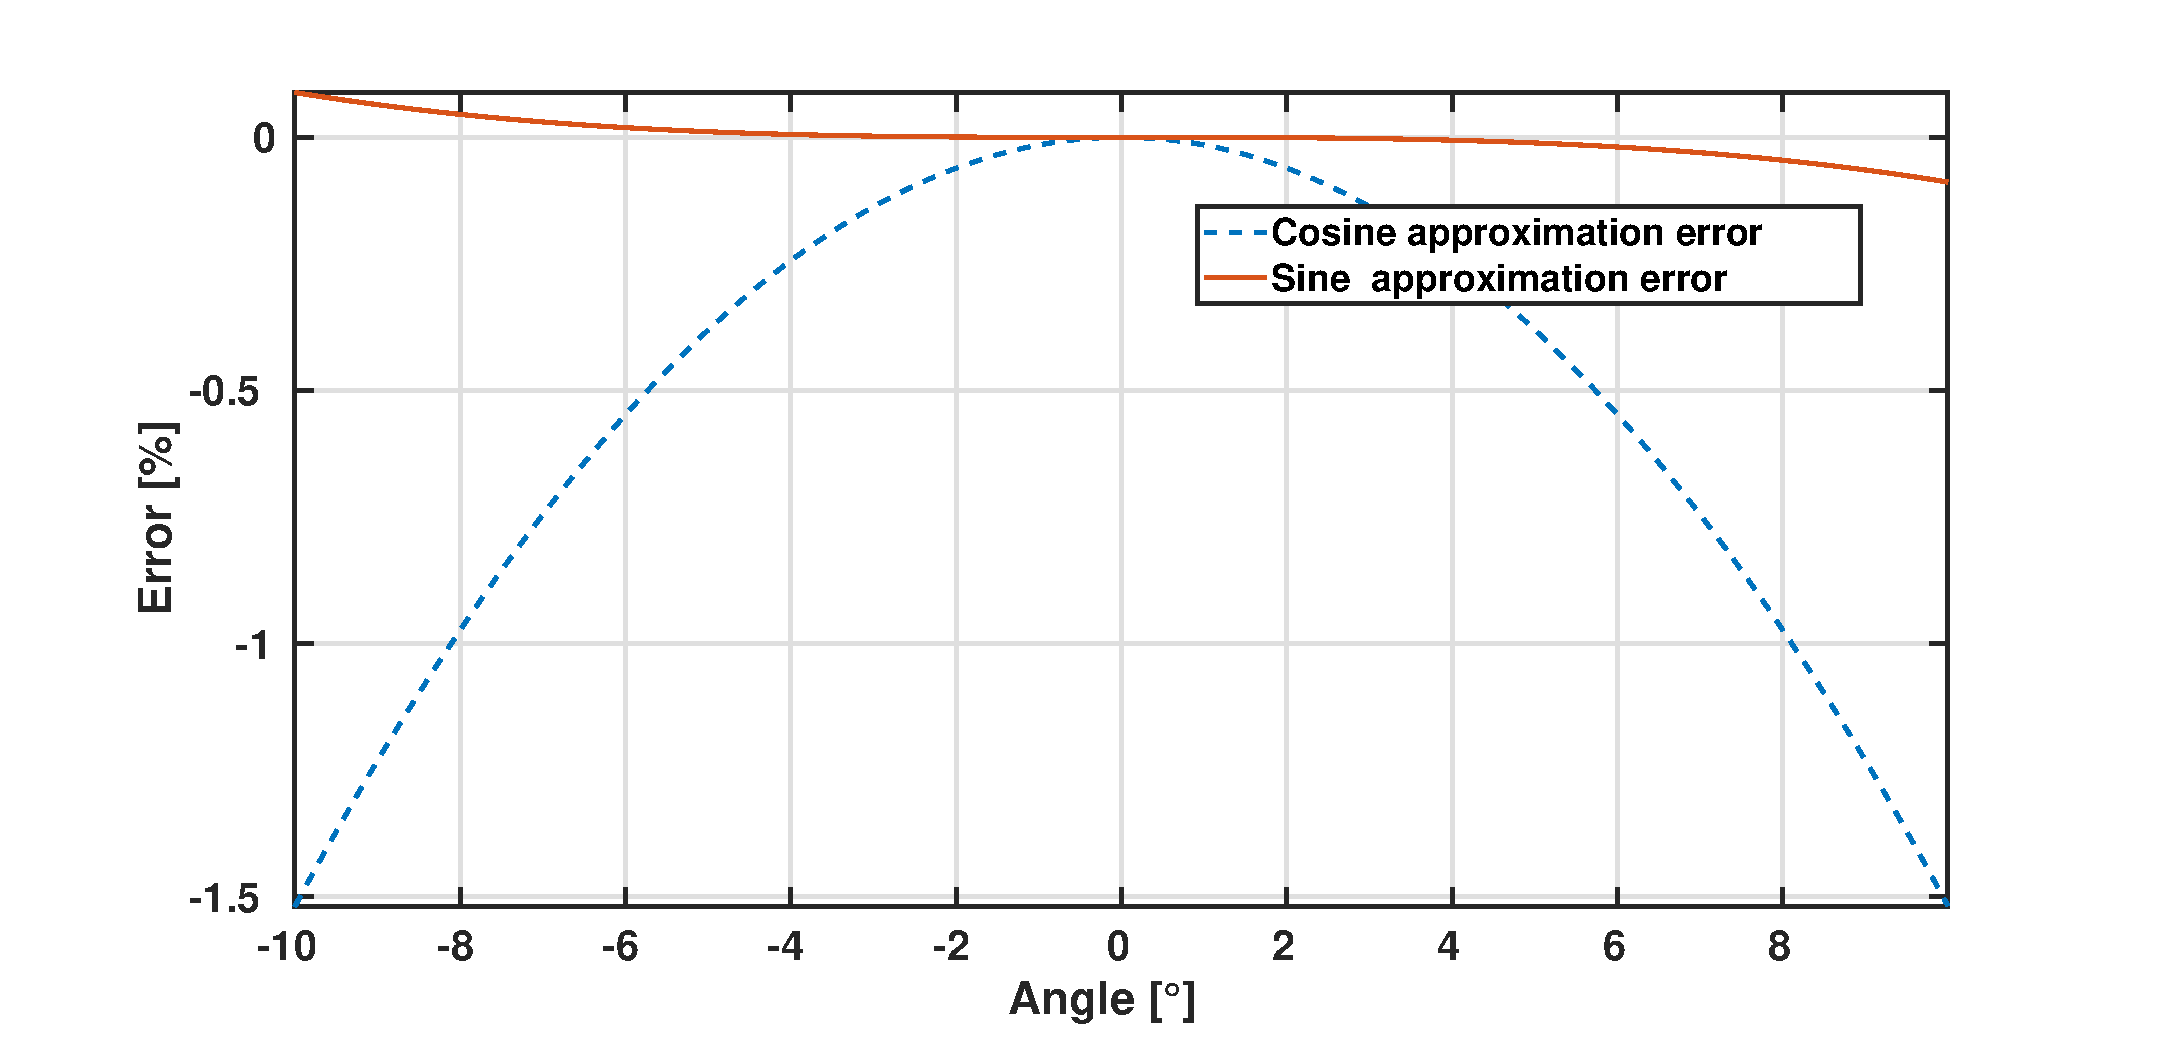
\includegraphics[width=0.8\textwidth]{CosSinLinApprox}
	\caption{Error generated by the approximation of the cosine and the sine function}\label{fig:BasLinPlot}
\end{figure}